\documentclass[12pt,a4paper]{article}
\usepackage{oeNIKstyle}

\usepackage[utf8]{inputenc}

\usepackage{float}
\usepackage{graphicx}
\usepackage{subfig}
\usepackage[titletoc]{appendix}
\usepackage{pdfpages}
\usepackage{subfig}
\usepackage{graphicx}
\usepackage{hyperref}
\hypersetup{
	colorlinks=true,
	linkcolor=blue,
	filecolor=magenta,      
	urlcolor=cyan,
}

\usepackage{minted}
\usemintedstyle{tango}
\usepackage{verbatim}

%\usepackage[T1]{fontenc}
\usepackage[magyar]{babel} % magyarra nyelvi csomag

\setlength{\parindent}{0 mm} % behúzás mértékét állíthatjuk be


\author{Gipsz Jakab}
\torzsKonyvSzam{T/xxxxxx/xxxxxx/x}
\neptunNumber{HTKMNE}

% lehetne egy változóban, de akkor nem tudjuk kontrolállni, hogy hogyan legyen megtörve.
\hunTitleFirstRow{Szoftver megoldás fejlesztése rendezetlen alkatrészek}
\hunTitleSecondRow{robotizált manipulációjára}

\engTitleFirstRow{Development of a software solution for robotized handling}
\engTitleSecondRow{of assoreted components}

\supervisor{Dr. Galambos Péter}
\consultant{???}

\deadlineDate{2020. május 22.}
\terminationDate{2021. május 22.}

% set the page style
\makedefaultpagestyle

%TODO hivatkozások előtt space-t hagyni
%TODO képeknél hivatkozást zárójelbe rakni: (Forrás:cite)
%TODO XMl szekvencia diagram készítése a teljes folyamat leírására
%TODO hivatkozások javítása

\begin{document}
	\maketitle
	\makeassigmentpage
	% a feladat és a tartalmazandók listája a lennti két fájlból töltendő be
	\makeassigmentpagetwo{theassigment}{themustbeinassigment}
	\makedeclaration
	\setcounter{page}{1} % start counting pages from here
	
	\maketoc
	
	\section{Bevezetés}
	A dokumentum célja, hogy kiindulópontot adjon a szakdolgozat és diplomamunka elkészítéséhez LaTex-ben környezetben. 
	
	Itt szándékosan elhelyezünk egy oldaltörést\footnote{mert megtehetjük}.
	\pagebreak
	
	\section{Ábrák}
	
	\begin{figure}[h!]
		\centering
		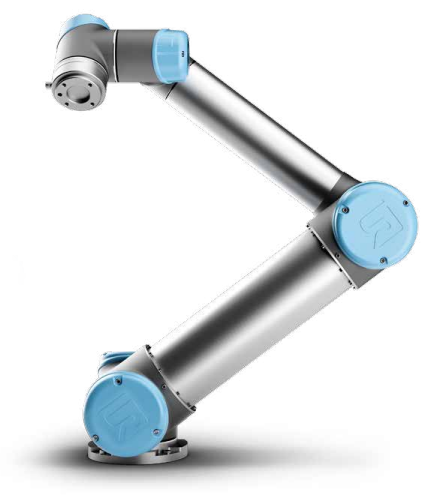
\includegraphics[width=0.5\linewidth]{img/ur5robot.png}
		\caption[UR5 Koolabortív robot]{UR5 Kollaboratív robot (forrás: http://universalrobots.com)}
		\label{fig:robotik-bin-picking}
	\end{figure}
	
	\section{Hivatkozások}
	
	Ez itt egy folyóirat cikk \cite{journal-example}.
	
	Ez itt egy konferencia cikk \cite{conference-example}.
	
	Ez itt egy könyv \cite{book-example}.
	
	Ez itt egy online forrás \cite{online-example}.
	
	Ez itt egy disszertáció \cite{thesis-example}.
	
	\section{Egyenletek}
	
	\section{Táblázatok}
	Példaként itt látható egy táblázat (\ref{tab:ur5}. Táblázat)
	
	\begin{table}[]
		\centering
		\caption{AZ UR5 robot főbb paraméterei}
		\label{tab:ur5}
		\begin{tabular}{l|l}
			Tulajdonság                      & Érték    \\ \hline
			kinyúlás {[}mm{]}                & 850      \\ \hline
			Szabadságfok                     & 6        \\ \hline
			Teherbírás {[}kg{]}               & 5        \\ \hline
			Súly {[}kg{]}                    & 18,4     \\ \hline
			Ismétlési pontosság {[}mm{]}     & $\pm0,1$    \\ \hline
			Teljesítményfelvétel {[}W{]}     & 90-325   \\ \hline
			Csuklók mozgástartománya {[}$^{\circ}${]} & $\pm360$    \\ \hline
			Max. csuklósebesség {[}$^{\circ}/sec${]}  & $\pm180$    \\ \hline
			Max. Tool sebesség {[}m/s{]}     & 1        \\ \hline
			Programozási nyelv               & URscript \\ \hline
		\end{tabular}
	\end{table}

	Egy másik táblázat.
	\begin{table}
	\centering
	\begin{tabular}{ccccc}
		Robotcsukló & \begin{tabular}[c]{@{}c@{}}min. poz.\\ {[}rad{]}\end{tabular} & \begin{tabular}[c]{@{}c@{}}max. poz.\\ {[}rad{]}\end{tabular} & \begin{tabular}[c]{@{}c@{}}max. sebesség\\ {[}rad/s{]}\end{tabular} & \begin{tabular}[c]{@{}c@{}}max. gyorsulás\\ {[}rad/s\textasciicircum{}2{]}\end{tabular} \\
		1 & -0.802 & 1.39 & 3.1 & 9 \\
		2 & -2.25 & -0.873 & 3.1 & 9 \\
		3 & 1.25 & 2.7 & 3.1 & 9 \\
		4 & -3.49 & -1.41 & 3.1 & 9 \\
		5 & -2.62 & -0.62 & 3.1 & 9 \\
		6 & -3.14 & 2.09 & 3.1 & 9
	\end{tabular}
	\caption{}
	\label{tab:joint-limits}
	\end{table}

	Táblázatok szerkesztésére számos online eszköz áll rendelkezésre. Ezek közül néhány:
	\begin{itemize}
		\item \href{https://www.tablesgenerator.com}{https://www.tablesgenerator.com}
		\item \href{https://www.latex-tables.com}{https://www.latex-tables.com}
		\item \href{https://tableconvert.com}{https://tableconvert.com}
	\end{itemize}


	Minden amit a LaTex táblázatokról tudni érdemes: https://www.overleaf.com/learn/latex/tables
	
	\section{Képletek}
	Ha egy képletet akarok bemutatni, akkor lássuk a \ref{eq:fig_akarmi} képletet:\\
    \begin{equation}
        \mathlarger{ % képlet növelés
        \cos{\alpha-\beta} = \cos{\alpha}\cdot\sin{\beta}-\cos{\beta}\cdot\sin{\alpha}}
        \label{eq:fig_akarmi}
    \end{equation}	
    
    Ha több sorosat, akkor meg a \ref{eq:fig_valami} képletet, ahol az egyenlőségjelek össze vannak rendezve \textbackslash \&=, és nincs rajta méretváltoztató utasítás.
    \begin{equation}
        %
        \begin{aligned}
        \cos{\alpha-\beta} \&= \cos{\alpha}\cdot\sin{\beta}-\cos{\beta}\cdot\sin{\alpha}\\
         \cos{\alpha}\cdot\sin{\beta}-\cos{\beta}\cdot\sin{\alpha} \&= \cos{\alpha-\beta}
        \end{aligned}
        \label{eq:fig_valami}
    \end{equation}	
    
    inline egyenlet lehet pl \(V_{max}=2 \), de lehet így is: \begin{equtation} \sqrt{a+b}\end{equtation}, izlés szerint. 

	\section{Egyéb szerkezetek}
	Néhány gyakran használt szerkezetet itt mutatunk be. Folyamatosan bővül.
	
	\subsection{Felsorolás}
		
		\begin{itemize}
			\item A felsorolás első eleme
			\item A felsorolás második eleme
			\item A felsorolás harmadik eleme
			\item ...
		\end{itemize}
	
		Szükség esetén kiemelhető az első szó.
		
		\begin{itemize}
			\item \textbf{revoulte:} tengely mentén forog, ennél a típusnál megadható alsó és felső határ
			\item \textbf{continuous:} tengely mentén forog, nincs alsó és felső határa
			\item \textbf{prismatic:} transzlációs csukló, tengely mentén mozog alsó és felső határ között
			\item \textbf{floating:} ez a csuklótípus lehetővé teszi a mozgást mind a 6 szabadsági fokban
			\item \textbf{fixed:} 0 szabadsági fokkal rendelkező csukló
		\end{itemize}
	
	\subsection{Számozott lista}
		
		\begin{enumerate}
			\item A számozott lista első eleme
			\item A számozott lista második eleme
			\item A számozott lista harmadik eleme
			\item ...
		\end{enumerate}
	
	\subsection{Forráskódok}	
	
	A \verb|minted| csomag segítségével tudunk kódokat beilleszteni. Első lehetőség a kód beillesztése a LaTex fileba: 
	
	\begin{minted}[
        frame=lines,
        framesep=2mm,
        baselinestretch=1.2,
        fontsize=\footnotesize,
    linenos]{c++}
		std::vector<std::pair<double, geometry_msgs::Transform>> partDistList;
		partDistList.resize(lastPickPoseVect.size());
		int counter = 0;
		double distance = 0.0;
		for(auto it = lastPickPoseVect.begin(); it != lastPickPoseVect.end(); it++) {
			tf::Transform tmpPose;
			tf::transformMsgToTF(*it, tmpPose);
			distance = lastPickPose.getOrigin().distance(tmpPose.getOrigin());
			// put the distance and the pose to the partDistList
			partDistList[counter].first = distance;
		partDistList[counter].second = *it;
		counter++;
		}
	\end{minted}
	
	Sokszor azonban kényelmesebb behivatkozni:
	
	\inputminted{c++}{code/example.cpp}
	
	A  \verb|minted| egy nagyon szofisztikált csomag, rengeteg beállítással. A teljes dokumentáció \href{https://ctan.org/pkg/minted?lang=en}{itt} érhető el.
	
	
    \makebibliography
	\makefigures
	\maketables
	
	\appendix
	
	\section*{Függelék}
	\begin{appendices}
		\section{ur-ros-state-server} 
		\label{appendix:ur-ros-state-server}
		\inputminted{js}{code/ur5_state_server.js}
		
		\pagebreak
		
		\section{ur\_5\_upload}
		\label{appendix:ur_5_upload}
		\inputminted{xml}{code/ur5_upload.launch}
	\end{appendices}
\end{document}

